\chapter{常用的python模块}
\section{Argparse}
argparse模块是一个用户用户友好的命令行接口,当用户每有给定可用的参数时,argaprser能自动生成帮助和使用信息。
\begin{python}
import argparse
parser = argparse.ArgumentParser(description='Process some integers.')
parser.add_argument('integers',metavar='N',type=int,nargs='+',help='an integer for the accumulator')
parser.add_argument('--sum',dest='accumulate',action='store_const',const=sum,default=max,help='sum the integers(default:find the max)')
args = parser.parse_args()
print(args.accumulate(args.integers))
\end{python}
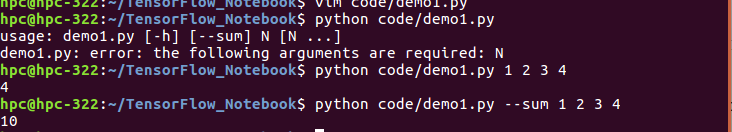
\includegraphics[scale=0.5]{demo1.png}
\begin{python}
代码能根据传入的参数选择相应的函数计算。
\begin{itemize}
\item 创建一个parser
\item 增加arguments
\item 解析参数
\end{itemize}
\subsection{ArgumentParser 对象}
class argparse.ArgumentParser(prog=None, usage=None, description=None, epilog=None, parents=[], formatter\_class=argparse.HelpFormatter, prefix\_chars='-', fromfile\_prefix\_chars=None, argument\_default=None, conflict\_handler='error', add\_help=True, allow\_abbrev=True)
\begin{itemize}
\item prog:程序的名字(默认为sys.argv[0])
\item usage:描述程序用法的字符串。(默认同感arguments增加到parser)
\item description:argument帮助前的文本展示。(默认为:None)
\item epilog:argument帮助之后的文本展示。(默认为:None)
\item parents:应该被包含的列表对象。
\item formatter\_class:自定义输出帮助的类。
\item prefix\_chars:参数前面的字符。(默认为'-')
\item fromfile\_prefix\_chars:应该被读的文件的字符串。
\item argument\_default:参数的全局值。(default:None)
\item conflict\_handler:解决冲突选项的策略。(通常不是必需的)
\item add\_help:增加-h/--help选项到parser。(默认为True)
\item allow\_abbrev:如果缩略不冲突,可以允许长的选项被缩略。(默认为True)
\end{itemize}
\subsection{prog}
默认情况下ArgumentParser对象用sys.argv[0]决定如何显示程序的名字。

#filename:arg1.py
import argparse
parser = argparse.ArgumentParser()
parser.add_argument("echo")
args = parser.parse_args()
print(args.echo)
\end{python}
输入:\newline
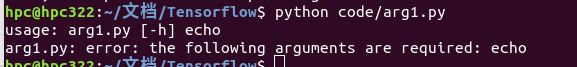
\includegraphics[scale=0.5]{arg1.png}\newline
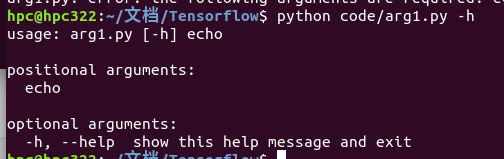
\includegraphics[scale=0.5]{arg2.png}\newline
add\_argument方法指定程序需要接受的命令参数,本例中为echo,此程序运行必须指定一个参数,方法parse\_args()同感分析指定的参数返回数据echo。
\begin{python}
import argparse
parser = argparse.ArgumentParser()
parser.add_argument("echo",help="show the help information",type=int)
args = parser.parse_args()
print(args.echo**2)
\end{python}
指定参数类型为int,默认为string。
\begin{python}
import argparse
parser = argparse.ArgumentParser()
parser.add_argument("--verbosity",help="increase output verbosity")
args = parser.parse_args()
if args.verbosity:
    print("Verbosity turned on")
\end{python}

\includegraphics[scale=0.5]{arg3.png}\newline
这里指定了--verbosity程序就显示一些信息,如果不指定程序也不会出错,对应的变量就被设置为None。
\begin{python}
import argparse
parser = argparse.ArgumentParser()
parser.add_argument("--verbosity",help="increase output verbosity",action="store_true")
args = parser.parse_args()
if args.verbosity:
    print("Verbosity turned on")
\end{python}
指定一个新的关键词action,赋值为store\_ture。如果指定了可选参数,args.verbose就赋值为True,否则就为False。
\begin{python}
import argparse
parser = argparse.ArgumentParser()
parser.add_argument("-v","--verbose",help="Increase output verbosity",action="store_true")
args = parser.parse_args()
if args.verbose:
    print("verbosity turned on")
\end{python}
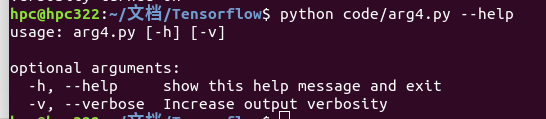
\includegraphics[scale=0.5]{arg4.png}\newline
\begin{python}
#args5.py
import argparse
parser = argparse.ArgumentParser()
parser.add_argument("square",type=int,help="display help information")
parser.add_argument("-v","--verbose",action="store_true",help="increase output verbosity")
args = parser.parse_args()
answer = args.square**2
if args.verbose:
    print("The square of {} equals {}".format(args.square,answer))
else:
    print(answer)
\end{python}
输入参数--verbose和整数(4)顺序不影响结果。
python args5.py --verbose 4和python args5.py 4 --verbose
\begin{python}
import argparse
parser = argparse.ArgumentParser()
parser.add_argument("square",type=int,help="display a square of a given number")
parser.add_argument("-v","--verbosity",type=int,help="increase output verbosity")
args = parser.parse_args()
answer = args.square**2
if args.verbosity == 2:
    print("The square of {} equals {}".format(args.square,answer))
elif args.verbosity == 1:
    print("{}^2=={}".format(args.square,answer))
else:
    print(answer)
\end{python}
python args6.py 4 -v 0,1,2通过指定不同的参数v为0,1,2得到不同的结果。
\begin{python}
#arg7.py
import argparse
parser = argparse.ArgumentParser()
parser.add_argument("square",type=int,help="display the square of a given number")
parser.add_argument("-v","--verbosity",action="count",help="increase output verbosity")
args = parser.parse_args()
answer = args.square**2
if args.verbosity == 2:
    print("The square of {} equals {}".format(args.square,answer))
elif args.verbosity == 1:
    print("{}^2 == {}".format(args.square,answer))
else:
    print(answer)
\end{python}
这里添加参数action="count",统计可选参数出现的次数。
python arg7.py 4 -v(出现一次),对应结果为x\^{}2 == 16\newline
python arg7.py 4 -vv(出现两次),对应出现The square of 4 equals 16\newline
\begin{python}
import argparse
parser = argparse.ArgumentParser()
parser.add_argument("square",type=int,help="display a square of a given number")
parser.add_argument("-v","--verbosity",action="count",default = 0,help="increase output verbosity")
args = parser.parse_args()
answer = args.square**2
if args.verbosity>=2:
    print("The square of {} equals {}".format(args.square,answer))
elif args.verbosity>=1:
    print("{}^2 == {}".format(args.square,answer))
else:
    print(answer)
\end{python}
加速让default参数。这只默认为值0,当参数v不指定时参数就被置为None,None不能和整型比较。
\begin{python}
import argparse
parser = argparse.ArgumentParser()
parser.add_argument("x",type=int,help="The base")
parser.add_argument("y",type=int,help="The exponent")
parser.add_argument("-v","--verbosity",action="count",default=0)
args = parser.parse_args()
answer = args.x**args.y
if args.verbosity >=2:
    print("{} to the power {} equals {}".format(args.x,args.y,answer))
elif args.verbosity >=1:
    print("{}^{} == {}".format(args.x,args.y,answer))
else:
    print(answer)
\end{python}
为了让后面的参数不冲突,我们需要使用另一个方法:
\begin{python}
#args10.py
import argparse
parser = argparse.ArgumentParser()
group = parser.add_mutually_exclusive_group()
parser.add_argument("-v","--verbose",action="store_true")
group.add_argument("-q","--quit",action="store_true")
parser.add_argument("x",type=int,help="The base")
parser.add_argument("y",type=int,help="The exponent")
args = parser.parse_args()
answer = args.x**args.y
if args.quit:
    print(answer)
elif args.verbose:
    print("{} to the power {} equals {}".format(args.x,args.y,answer))
else:
    print("{}^{} == {}".format(args.x,args.y,answer))
\end{python}
可以输入python arg10.py 3 4 -vq得到计算结果。
\begin{python}
import argparse
parser = argparse.ArgumentParser()
group = parser.add_mutually_exclusive_group()
group.add_argument("-v","--verbose",action="store_true")
group.add_argument("-q","--quit",action="store_true")
parser.add_argument("x",type=int,help="The sase")
parser.add_argument("y",type=int,help="The exponent")
args = parser.parse_args()
answer = args.x**args.y
if args.quit:
    print(answer)
elif args.verbose:
    print("{} to the power {} equals {}".format(args.x,args.y,answer))
else:
    print("{}^{} == {}".format(args.x,args.y,answer))
\end{python}
这里参数v和q不能同时使用。

